\setlength\abovedisplayskip{0.4pt}
\setlength\belowdisplayskip{0.4pt}

\chapter{Ultra-peripheral collisions and photoproduction}

In this chapter, we will review recent LHC results on ultra-peripheral collisions (UPCs). First we will discuss the unique features of UPCs, and how they are selected. We then present the results from ALICE and CMS on vector meson photoproduction as an example of how UPCs can probe the nuclear gluon distribution. The ATLAS results for light-by-light scattering are also described. The final section explains dijet photoproduction in UPCs, and how the factorisation theorem informs the interpretation of coherent dijet correlation. Finally, we present the physics motivation to study the angular correlation of UPC dijet, which is the analysis presented in this thesis. 

\section{Ultra-peripheral heavy-ion collisions}

Ultra-peripheral collisions occur at impact parameters greater than the sum of the heavy-ion radii. In these collisions, hadronic interactions are strongly suppressed while photonuclear activity is enhanced proportional to the square of the nuclear charge \cite{Contreras:2015dqa}. The electromagnetic field of an incoming heavy-ion, from the perspective of a target, is equivalent to a flux of virtual photons; Figure \ref{fig:smushedField} illustrates the Lorentz contraction of the field of a boosted charge \cite{Baltz:2007kq,WWJackson}.

\begin{figure}[h!]
\begin{centering}
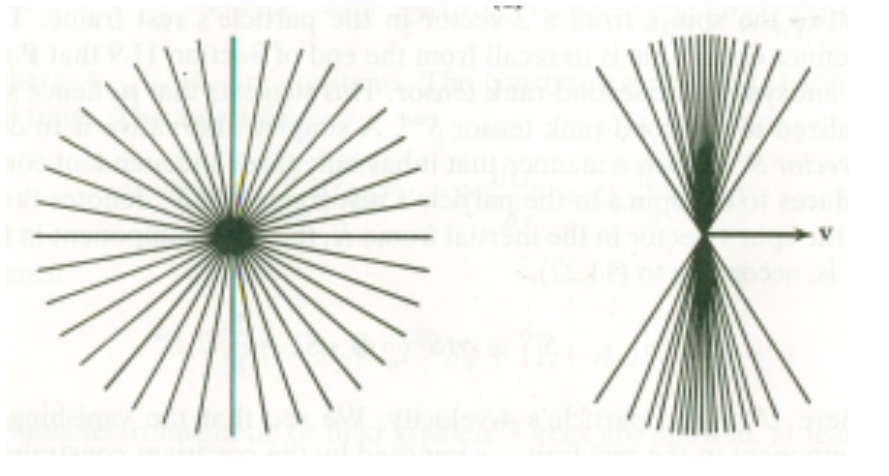
\includegraphics[width=4in]{Chapter1/importfigs/jackson_em_wwa.png}
\par\end{centering}
\caption{ (a.) electromagnetic field of stationary charge (b.) eletromagnetic field of boosted charge \cite{WWJackson} \label{fig:smushedField}}
\end{figure}

UPC models typically address two elements: the photon flux, $N_{\gamma / Pb}$, and the photoproduction cross-section, $\sigma_{\gamma Pb}$. These quantities are related to the UPC cross-section, $\sigma_{PbPb}$, in the following equation
\begin{equation}
\frac{d \sigma_{PbPb}}{dy} = N_{\gamma/Pb}(y,M)\sigma_{\gamma Pb}(y)+N_{\gamma/Pb}(-y,M)\sigma_{\gamma Pb}(-y),
\end{equation}
where there are two terms to reflect that either heavy-ion can be a source of photons \cite{Bertulani:2005ru}. 

The Weizsacker-Williams appoximation (WWA) calculates the density of photons, about the nucleus, as a function of energy. WWA is a semi-classical formulation. Maxwell's equations are solved for a stationary point charge boosted to an ultra-relativistic velocity. In the target's frame, the Fourier transform of the source field is taken. The Fourier frequency modes are interpreted through the quantum mechanical equation of photon energy. The photon flux as function of energy is given by
\begin{equation}
N(\omega,b) = \frac{\alpha}{\hbar \omega}\left( \frac{Z}{b\beta\pi} \right)^2\left ( \frac{\omega b}{\gamma \nu} \right )K_1^2\left ( \frac{\omega b}{\gamma \nu} \right ) ,
\end{equation}
where $\alpha$ is the QED coupling constant, $\omega$ is the photon energy, $Z$ is the atomic number of the nuclei, $b$ is the impact parameter, $\beta$ is the ratio of the nuclei speed to the speed of light, $\gamma$ is the Lorentz boost of the nuclei, $K_1^2$ is a Bessel function, and $\nu$ is the photon frequency \cite{WWJackson}.

The photon flux can be written as a function of the photon wavelength:
\begin{equation}
n(k) = \frac{2 \alpha Z^2}{\pi}\left [ \xi K_0(\xi) - \frac{\xi^2}{Z}(K_1^2(\xi)-K_0^2(\xi)) \right ]
\end{equation}

For a given final state $X$, the collision cross section is given as
\begin{equation}
\sigma_X = \int d \omega \frac{n(\omega)}{\omega} \sigma_X^\gamma(\omega),
\end{equation}
where $n(\omega)$ is the number of photons emitted at an energy $\omega$, and $\sigma_X^\gamma(\omega)$ is the photonuclear cross-section of the photon-nucleon interaction. The Weizacker-Williams approximation provides $n(\omega)$. The integral reflects how a state $X$ can result from the interaction of a quasi-real photon of varying energy \cite{Nystrand:2004vn}. At low momentum transfer, photons interact electromagnetically, i.e. directly, with partons \cite{photonALICE}. High energy, "resolved" photons possess a hadronic structure; instead of directly interacting with the nuclei, these photons fluctuate into mediating quark-antiquark pairs.

UPCs can generate a wide variety of particles. In the next section we will discuss current results on vector meson photoproduction.

\section{VM photoproduction}
The vector mesons are a subset of the mesons that have spin-1 and negative parity. There are three vector mesons that have recently been studied in UPCS: the $\rho^0$, the $J/\psi$, and the $\Upsilon(1S)$. The $\rho^0$ is an antisymmetric superposition of up and down quark-antiquark pairs, $(1/\sqrt{2})(u\bar{u}-b\bar{b})$. The $J/\psi$ consists of a charm quark and a charm antiquark. The $\Upsilon(1S)$ consists of a bottom quark and a bottom antiquark. $J/\psi$ and its excited states are referred to as charmonia; likewise, $\Upsilon(1S)$ and its excited states are referred to as bottomonia.

The Bjorken-$x$ probed by a specific UPC vector meson is set by the mass $M_{VM}$, the rapidity $y$, and collision energy $\sqrt{s}$, such that
\begin{equation}
x = \frac{M_{VM}}{\sqrt{s}}e^{\pm y}.
\end{equation} The vector meson mass also sets the hard scale, $Q^2$, of the photoproduction. For example, for the $J/\psi$
\begin{equation}
Q^2 = \frac{M_{VM}}{4}.
\end{equation}

The virtual photons present in UPC can fluctuate into a quark-antiquark pair which can take the form of a low mass meson \cite{lta2011.09,Chekanov:2002xi,Klasen:2007pm}. This meson then interacts with the target nuclei via colorless gluon exchange, emitting a vector meson \cite{Emling:1994gu,dePassos:2001dc,Ryskin:1992ui,Goldhaber:1948zza}. If the virtual photon interacts coherently with the target nucleus, this is reflected in the transverse momentum of the vector meson \cite{Goncalves:2011vf}. The vector meson decays into a dilepton pair that can be detected by the experiment. STARLIGHT is a Monte Carlo generator designed to model vector meson photoproduction in UPC \cite{starlight}.

\begin{figure}[h!]
\begin{centering}
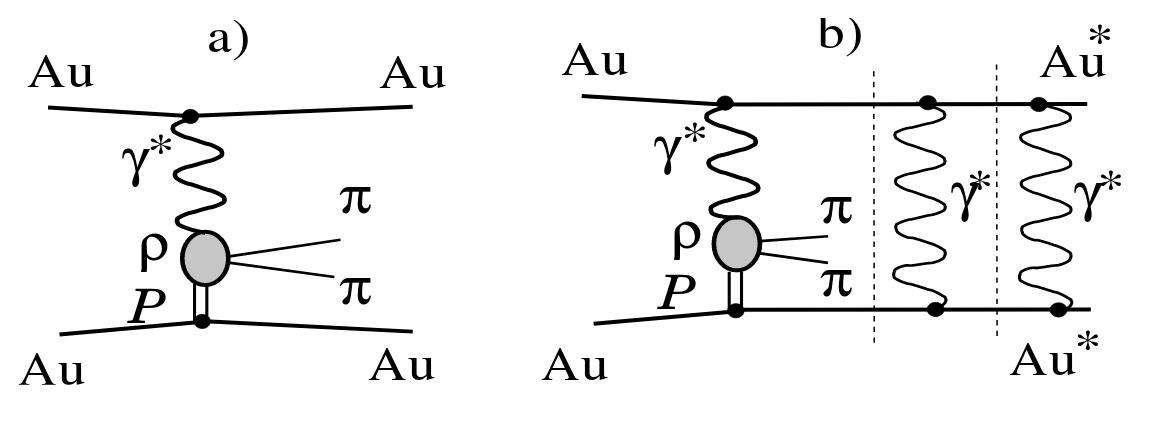
\includegraphics[width=5.5in]{Chapter2/importfigs/upc_star_diagram.png}
\par\end{centering}
\caption{$AuAu \rightarrow AuAu\rho^o$, (a.) UPC exclusive $\rho^o$ diagram, (b.) with mutual nuclei excitation \cite{Adler:2002sc} \label{fig:upcRhoStar}}
\end{figure}

One of the first observations of vector meson photoproduction in UPC was that of exclusive coherent $\rho^0$ production at STAR. For this process the source nuclei emits a virtual photon that fluctuates into a $\rho^0$ meson that scatters elastically off the target nuclei. The $\rho^o$ decays into a pair of oppositely charged pions. These pions leave two back-to-back tracks in the STAR tracker. The Feynman diagrams for the process are seen in Figure \ref{fig:upcRhoStar}. In exclusive production there are only two tracks in the tracker, with the rest of the detector being empty. In mutual nuclei excitation, the further exchange of virtual photons excite both nuclei and produce tracks in addition to those of the dipion system. The exclusive events were selected by STAR using a low-multiplicity trigger, while the mutual excitation events were selected using a minimum bias trigger with the additional requirement of neutron emission detected in both ZDCs \cite{Adler:2002sc}. 

One of the key signatures of coherent $\rho^0$, and UPC coherent mesons in general is the low-$p_T$ peak of the vector meson. If the virtual photon has energy on the order of $1/2R_{A}$, where $R_{A}$ is the radius of the nuclei, the photon couples with the whole nucleus. The low momentum corresponds to large wavelength of the photon with respect to the nuclear radius \cite{Guzey:2013taa,Frankfurt:2006wg,Baltz:2002pp,Klein:2003vd}. The $p_T$ spectrum of the $\rho^0$ detected by the topology and minimum-bias triggers are shown in Figure \ref{fig:upcRhoStarPt}, where the low $p_T$ $\rho^0$ candidates consistent with coherent photoproduction are seen for the two different triggers.

\begin{figure}[h!]
\begin{centering}
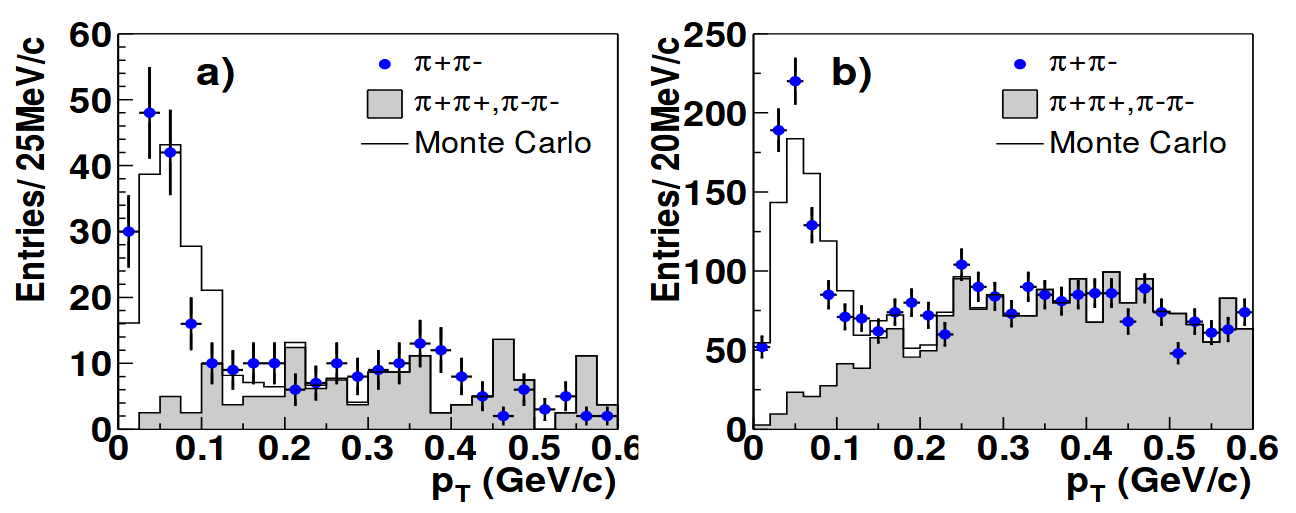
\includegraphics[width=5.5in]{Chapter2/importfigs/rho_upc_pt_star.png}
\par\end{centering}
\caption{UPC exclusive $\rho^o$ $p_T$, (a.) topology triggered (b.) minimum bias triggered \cite{Adler:2002sc} \label{fig:upcRhoStarPt}}
\end{figure}

More recently, ultra-peripheral coherent $J/\psi$ photoproduction was studied by the ALICE Collaboration using the 2011 Pb-Pb data \cite{Abelev:2012ba}. Notice that the cross section of coherent $J/\psi$ photoproduction, for $\gamma+p\rightarrow J/\psi+p$, has a power-law dependence on the photon-proton center-of-mass energy, as seen in Figure \ref{fig:aliceData1} \cite{Klein:2017nqo}. This data can be is sensitive to the gluon distribution in the proton as a function of Bjorken-$x$ \cite{pQCD2011.08}.

\begin{figure}[h!]
\begin{centering}
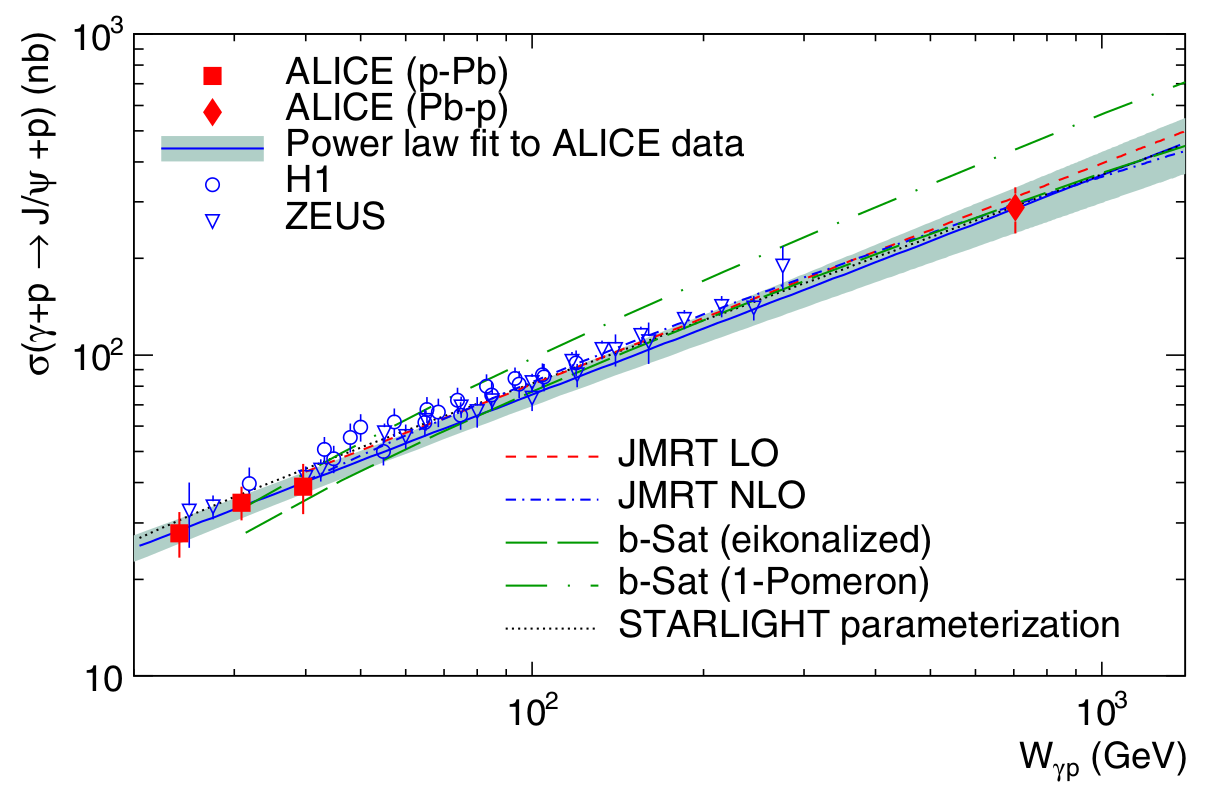
\includegraphics[width=3.5in]{Chapter2/importfigs/alice_jpsi_data.png}
\par\end{centering}
\caption{$\gamma +$proton$\rightarrow J/\psi +$proton cross section, showing the ALICE and HERA data \cite{Klein:2017nqo}. \label{fig:aliceData1}}
\end{figure}

CMS and ALICE have studied $J/\psi$ and $\rho^0$ photoproduction off the proton in proton-Pb collisions \cite{TheALICE:2014dwa}. In coherent UPC photoproduction of $J/\Psi$, the transverse momentum distribution peaks at about 60 MeV because, for coherent production, the photon energy is inversely proportional to the Pb ion diameter, $1/2R_{Pb}$.

\begin{figure}%
    \centering
    \subfloat[]{{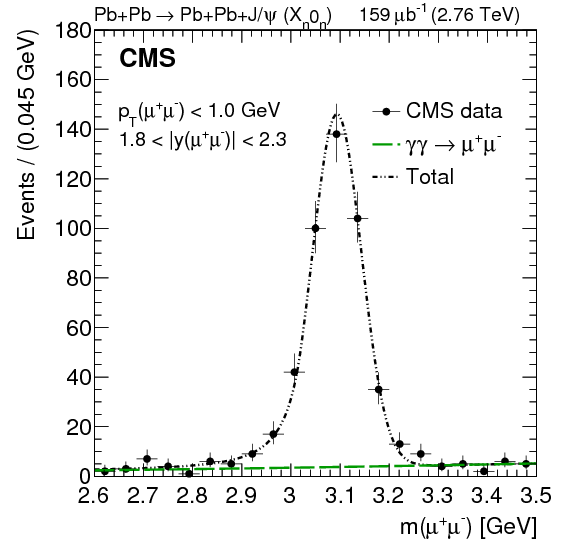
\includegraphics[width=7.cm]{Chapter2/importfigs/patkenny_Figure_001-a.png} }}%
    \qquad
    \subfloat[]{{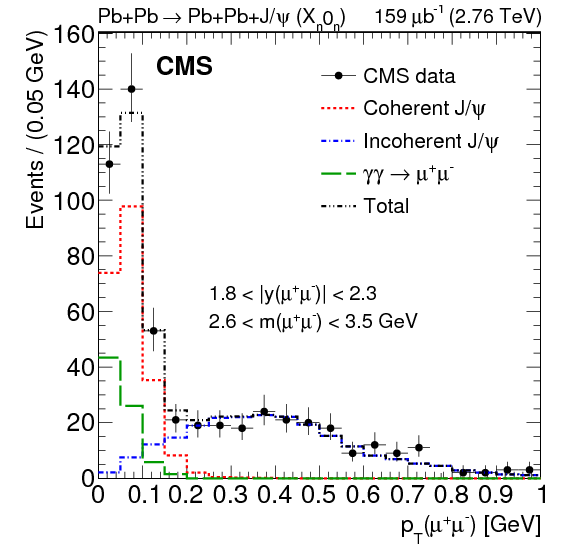
\includegraphics[width=7.cm]{Chapter2/importfigs/patkenny_Figure_001-b.png} }}%
    \caption{(a) dimuon invariant mass spectrum, (b) dimuon $p_T$ spectrum for $J/\psi$ candidates \cite{Khachatryan:2016qhq}.}%
    \label{fig:patKennyPlots}%
\end{figure}

UPC vector mesons are a clean probe of the nuclear initial state \cite{Aktas:2006qs,oniaPol}. The high temperature environment of heavy-ion collisions produces a near viscosity free medium that exhibits collective flow. However, collective flow phenomena are also observed in heavy-ion collisions below the QGP phase transition. A good understanding of the heavy-ion initial state, before the phase transition, is necessary to detect authentic QGP pheneomena. UPC phenomena is sensitive to the initial state, as will be discussed below \cite{vmd1999,vmd2000.03}. 

The UPC $J/\psi$ in particular is senstive to the gluon distribution at low Bjorken-x in the hadron target \cite{Teubner:2005sj}. The UPC $J/\psi$ photoproduction cross section can be calculated from a Glauber model of the heavy-ion \cite{Brodsky:1994kf}. The impulse approximation depicts the nucleus as a sum of protons and neutrons by scaling up the photon-nuclear cross section derived from electron-proton collisions at HERA \cite{Miller:2007ri}. Forward neutron tagging was used to separate the coherently and incoherently produced $J/\psi$ \cite{Guzey:2013jaa,Strikman:2005ze,lta2012.03,emPcite4,emPCite5,emPCite6,upcNeuPHENIX}.

\begin{figure}[h!]
\begin{centering}
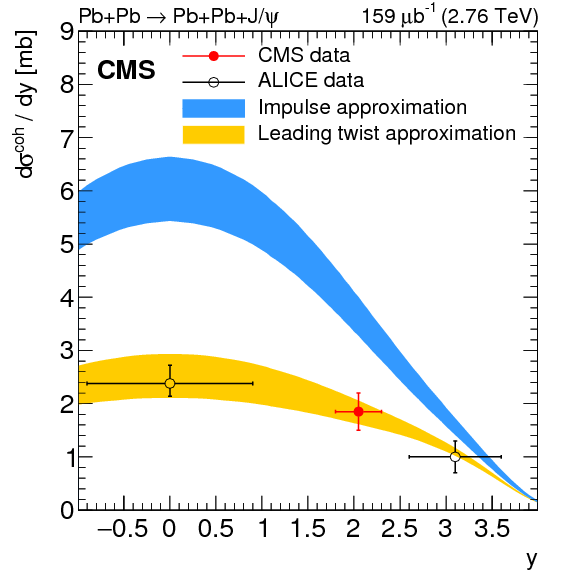
\includegraphics[width=3.5in]{Chapter2/importfigs/patkenny_Figure_002.png}
\par\end{centering}
\caption{Differential cross section versus rapidity for coherent $J/\psi$ photoproduction in ultra-peripheral PbPb collisions at $\sqrt{s_{NN}}=2.76$ TeV. Data are compared to theories incorporating the impulse approximation and the leading twist approximation \cite{Khachatryan:2016qhq}. \label{fig:pk3}}
\end{figure}

Studies of UPC $J/\psi$ at CMS show that the measured cross section is consistent with models of the nucleus that include moderately strong gluon shadowing, in particular EPSO9 \cite{lta2013.05,Eskola:2009uj}. Fig \ref{fig:pk3} compares the cross section measured by CMS and ALICE against theoretical models. In the data there is a clear difference from the Glauber model prediction. The cross sections indicate that, at the energy scale of the $J/\psi$ mass, the nuclear gluon density is suppressed with respect to that of the proton \cite{Frankfurt:2011cs}. Further studies can be done using UPC $\Upsilon$ \cite{pQCD2013.02,Cisek:2012yt}. 

\section{Photon-photon interactions}

Apart from vector meson photoproduction, in UPCs photon-photon interactions also occur. Classical electrodynamics forbids the scattering of a photon off another photon. According to Maxwell's equations, charge and current distributions make linear contributions to the electric and magnetic fields. For example, the electric field generated by a grid of static charges is the sum of the electric fields of each charge. This property is called the "principle of superposition", and allows Maxwell's equations to be solved as boundary values problems via the separation of variables.

The cross section of a final state from the photon-photon interaction is given by
\begin{equation}
\sigma_X = \int d \omega_1 d \omega_2 \frac{n(\omega_1)}{\omega_2} \sigma_X^{\gamma\gamma}(\omega_1, \omega_2),
\end{equation}
where the subscripts $1$ and $2$ designate the quasi-real photons that are colliding and 
$\sigma_X^{\gamma\gamma}(\omega_1, \omega_2)$ is the cross-section of the final state from a collision of photons with energies $\omega_1$ and $\omega_2$. Notice that the total final state cross-section is an integral of the all the photon energies in the photon flux. 

Maxwell's equations, being a classical theory, do not take into account the quantum mechanical effects that manifest at the distance scales of sub-atomic particles. The polarization of the vacuum is one such consequence of quantum mechanics. Around a photon there is a cloud of particle-antiparticle pairs, appearing together and then annihilating each other after a time proportional to their energy. In so far as these particles have an electric charge, portions of the local area may carry a non-zero electric charge. Thus, two photons may scatter off each other in three possible exchanges: Diagrams for Delbrück scattering, photon splitting, and elastic light-by-light scattering. 

\begin{figure}[]
\begin{centering}
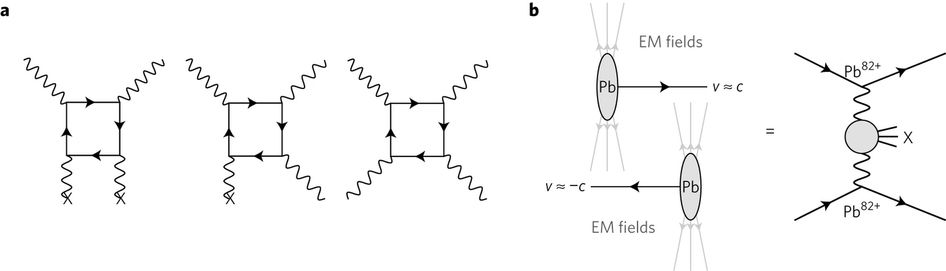
\includegraphics[width=7in]{Chapter2/importfigs/nphys4208-f1.jpg}
\par\end{centering}
\caption{Photon-photon diagrams of light-by-light scattering \cite{Aaboud:2017bwk}. \label{fig:ggDiag}}
\end{figure}

Figure \ref{fig:ggDiag} illustrates the process of light-by-light scattering. The plots in figure \ref{fig:ggDiag} (a.) are the Feynman diagrams of the three light-by-light channels: Delbruck scattering, photon splitting, and elastic scattering, respectively. Notice that all three channels are variations on a closed electron-loop. Figure \ref{fig:ggDiag} (b.) shows how these processes arise in heavy-ion collisions. The photon flux from a relativistic heavy-ion is calculated from the Fourier transform of its electric field. The final state $X$ is empty except for two photons \cite{Aaboud:2017bwk}. 

\begin{figure}[]
\begin{centering}
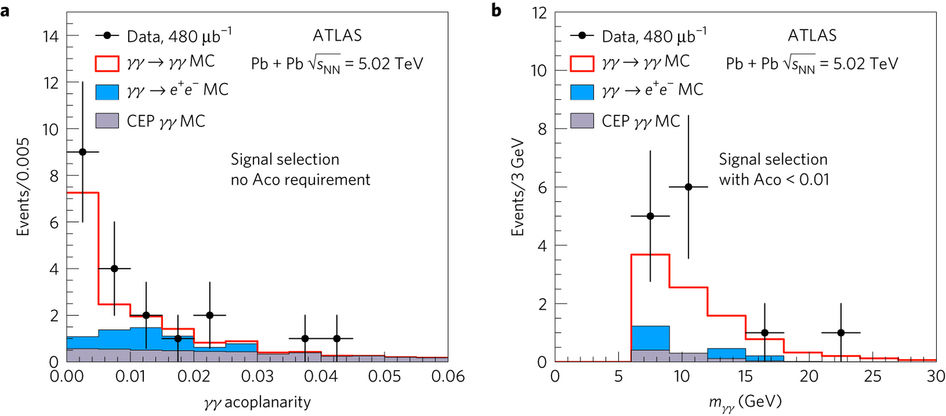
\includegraphics[width=7in]{Chapter2/importfigs/nphys4208-f3.jpg}
\par\end{centering}
\caption{$\gamma \gamma$ kinematics, (a.) acoplanarity, (b.) invariant mass \cite{Aaboud:2017bwk} \label{fig:ggKin}}
\end{figure}

Light-by-light scattering has been observed at ATLAS. The relevant data sample contains 480 $\mu b^-1$ of Pb+Pb data taken at $\sqrt{s_{NN}}=5.02$ TeV. Light-by-light MC was generated using STARLIGHT and processed through a GEANT4 simulation. The reconstructed MC was used to create kinematic templates for comparison against the data. These templates can be seen in figure \ref{fig:ggKin}. The most important part of the event selection is the requirement on diphoton acoplanarity. 

\section{Dijet photoproduction}

Jets are one of the most interesting nuclear phenomena discovered in the modern era of particle accelerators. The existence of jets is a direct result of QCD confinement. In hadron collisions, it is possible for the hadron's constituent partons to fragment away. However, QCD confinement -- caused by the running QCD coupling -- demands that only colorless objects can independently exist. Therefore, as the fragment partons separate, they manifest new partons around themselves and screen the color charge. The formation of colorless composites, out of colored partons, is called "hadronization". The process of hadronization continues until the kinetic energy of all the fragmented partons drops below the potential energy the binding strong force. The result is a narrow cone of hadrons fanning out from a common source: a "jet". Analyzing a jet can elucidate the properties of its mother parton \cite{d'Enterria:2004nv}.  

QCD factorisation describes the diffractive-photoproduction dijet cross-section as the convolution of the partonic cross-section with the diffractive parton distributions. However, factorisation only describes H1 data if the resolved-photon contribution is suppressed. 

Diffractive dijet photoproduction is not describable in perturbative QCD. For coherent processes the photon energy is small, and therefore the wavelength is large compared to the size of the nucleus. At these large distances, there is not a hard scale, and so perturbation calculations cannot be done. Gluon splitting interactions dominate the low Bjorken-x partons. QCD collinear factorization describes these soft interactions via the convolution of parton cross sections, taken from perturbative QCD, and diffractive parton distribution functions, taken from experiment \cite{Andreev:2015cwa,Chekanov:2008fh}. The photon can interact directly with the nucleon, or the photon can fluctuate into a quark-antiquark pair which interacts with the nucleon. The resolved-photon has a hadronic structure and its own corresponding PDF \cite{Bauer:1977iq}.

\begin{figure}[]
\begin{centering}
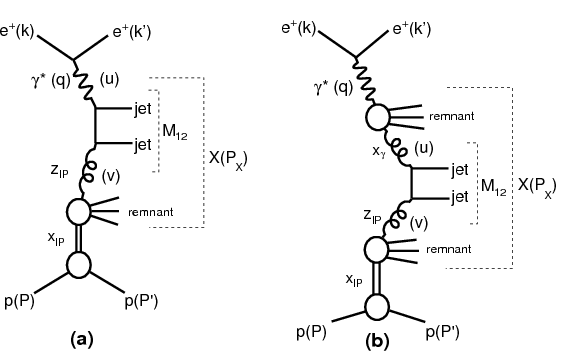
\includegraphics[width=6in]{Chapter1/importfigs/h1_2015_feyn.png}
\par\end{centering}
\caption{Feynman diagrams for coherent jet photoproduction in (a) direct-photon in ep interactions, (b) resolved-photon in ep interactions \cite{Andreev:2015cwa}. \label{fig:feynmanUPC1}}
\end{figure}

In electron-hadron collisions, diffractive photoproduction is characterized by the presence of a large rapidity gap in the final state and an intact nucleus \cite{Frankfurt:2006tp,Alexa:2013xxa,Aktas:2006qs}. The Feynman diagram of electroproduction in lepton-hadron collisions is similar to that of photoproduction in ultraperipheral collisions, as seen in Figure \ref{fig:feynmanUPC1} \cite{Andreev:2015cwa}. The large rapidity gap here is due to the leading proton \cite{Aaron:2010aa}. The diffractive dijet cross section is expressed by the convolution of partonic cross sections $d\hat{\sigma}$ and diffractive PDFs $f^D_{i/p}$.
\begin{equation}
d\sigma (ep \rightarrow e + 2 jets + X^{'} + p) = \sum_{i} \int dt \int dx_\mathbb{P} \int dz_\mathbb{P}d\hat{\sigma}_{ei\rightarrow 2jets}(\hat{s},\mu^2_R,\mu^2_F)\times f^D_{i/p}(z_\mathbb{P},\mu^2_F,x_\mathbb{P},t) ,
\end{equation}
where $x_\mathbb{P}$ is longitudinal momenetum fraction lost by the incoming proton, $d\hat{\sigma}_{ei\rightarrow 2jets}$ is the partonic cross-section for the process, $z_\mathbb{P}$ is the longitudinal momentum fraction of the Pomeron entering the hard process, $\hat{s}$ is the squared invariant energy of the subprocess, $\mu^2_R$ is the squared renormanlization scale, $\mu^2_F$ is the squared factorisation scale, $f^D_{i/p}$ is the diffractive parton distribution,and $t$ is the four-momentum transfer squared at the vertex. 

In the proton-vertex factorisation hypothesis, the dependence on $x_{\mathbb{P}}$ and $|t|$ is factored out of the dependence on $\mu^2_F$ and $z_{\mathbb{P}}$. Furthermore, $f^D_{i/p}$ is sum of contributions from the pomeron and Reggeon:
\begin{equation}
f^D_{i/p}(z_{\mathbb{P}},\mu^2_F,x_{\mathbb{P}},t) = f_{\mathbb{P}/p}(x_{\mathbb{P}},t)f_{i/\mathbb{P}}(z_{\mathbb{P}},\mu^2_F) + n_\mathbb{R}f_{\mathbb{R}/p}(x_{\mathbb{P}},t)f_{i/\mathbb{R}}(z_{\mathbb{P}},
\mu^2_F) ,
\end{equation}
where $_{\mathbb{P}/p}$ is the pomeron flux factor, $f_{\mathbb{R}/p}$ is the Reggeon flux factor, $n_\mathbb{R}$ is the normalization factor of the Reggeon, $f_{i/\mathbb{P}}$ is the pomeron parton distribution, and $f_{i/\mathbb{R}}$ is the Reggeon parton distribution. Figure \ref{fig:h1Ratio} compares the cross-section of H1 data to that predicted by NLO-QCD \cite{Andreev:2015cwa}.

\begin{figure}[h!]
\begin{centering}
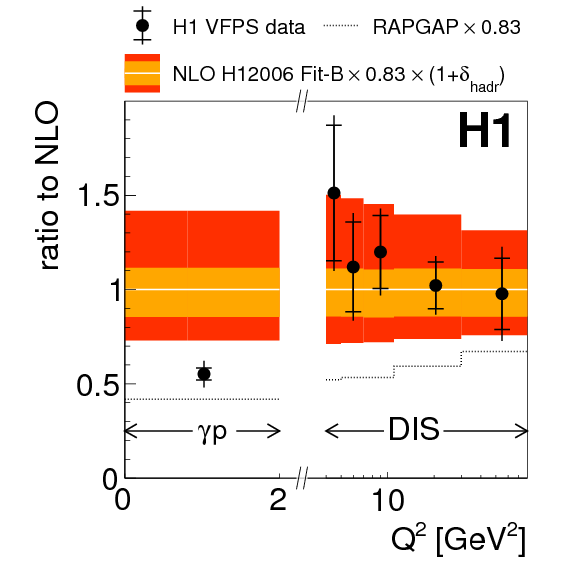
\includegraphics[width=3in]{Chapter1/importfigs/fig8_h1_2015.png}
\par\end{centering}
\caption{Ratio of H1 data cross-section to NLO-QCD cross-section \cite{Andreev:2015cwa}. \label{fig:h1Ratio}}
\end{figure}

H1 used the Very Forward Proton Spectrometer (VFPS) to trigger on low $Q^2$ protons. The VFPS consists of two Roman Pots located 218 m and 222 m from the H1 interaction-point in the forward direction. The VFPS can detect protons scattered at very low transverse momentum, corresponding to $0.008 < x_{P} < 0.028$ and $|t|<0.6$. Each of the Roman Pots contains layers of scintillating fibers, which are covered by a layer of scintillator tiles. The fibers readout to photomultipliers, and the tiles both shield from radiation and trigger on protons. The track effiency of VFPS is a remarkable $96 \%$, and the background contamination is kept at $1 \%$ , making the detector excellent for studying diffractive events \cite{Andreev:2015cwa}.


The H1 data was compared to predictions based on NLO-QCD convoluted with diffractive parton distribution functions (DPDFs) from HERA inclusive diffractive deep-inelastic scattering (DDIS) data. For diffractive pp collisions the high transverse momentum jets yield a hard scale for perturbative QCD \cite{Aaron:2010su}.

H1 used the RAPGAP MC generator to model diffractive $e+p \rightarrow e+X+p$ processes. The requirement of a leading proton, remaining intact or dissociating into a low energy state, was used to sample diffractive events. The collision product kinematics of data and MC are shown in figure \ref{fig:h1Kinematics}. Not only is the data in good agreement with predictions from RAPGAP, but the cross section of diffractive $e+p$ scattering is well described by calculations based on DPDFs. For this process, $\beta$ refers to the fraction of the pomeron's longitudinal momentum transferred to the parton within the nucleus \cite{Aaron:2010aa}. 

\begin{figure}[h!]
\begin{centering}
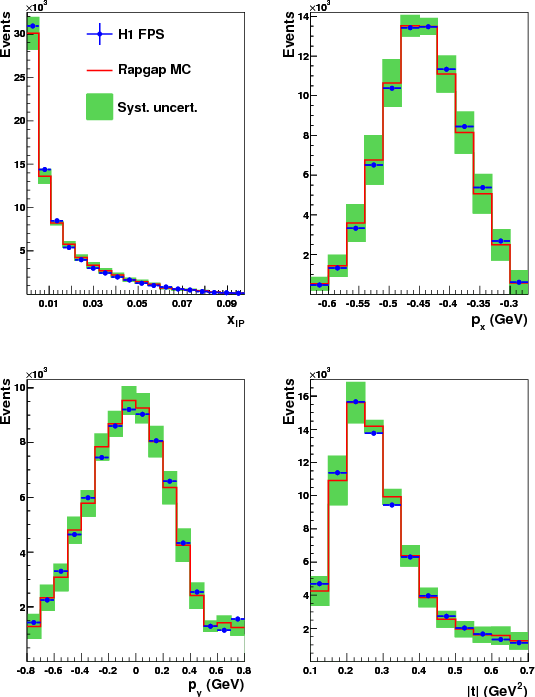
\includegraphics[width=4in]{Chapter2/importfigs/d10-095f3.png}
\par\end{centering}
\caption{H1, Diffractive $e+p$ products, Kinematics \cite{Aaron:2010aa} \label{fig:h1Kinematics}}
\end{figure}

\section{Wigner distribution}

The Wigner distribution was first developed as part of an attempt by Eugene Wigner to map solutions to Schr\"{o}dinger equation into phase probability distributions, i.e. a statistical mechanics interpretation of quantum mechanics.
\begin{equation}
\displaystyle P(x,p)~{\stackrel {\mathrm {def} }{=}}~{\frac {1}{\pi \hbar }}\int _{-\infty }^{\infty }\psi ^{*}(x+y)\psi (x-y)e^{2ipy/\hbar }\,dy\
\end{equation}
The Wigner distribution $P(x,p)$ can be used to calculate the expectation value of any given variable by considering the Wigner tranformation $g(x,p)$ of that variable's operator, $\hat{G}$,
\begin{equation}
\displaystyle \langle {\hat {G}}\rangle =\int \!dx\,dp~P(x,p)~g(x,p)~.
\end{equation}
Notice that in order to derive expectation values, the probability distribution most be integrated with respect to a function of position or momentum, which are still non-commuting according to the uncertainty principle. 

The Wigner distribution is a quantum phase space distribution that describes "elliptic" gluons \cite{Belitsky:2003nz}. Specifically, by considering the color diple scattering amplitude, the angular correlation of the nucleon recoil momentum and the dijet transverse momentum can provide a three-dimensional, tomographic image of the gluons within a high energy nucleus. This tomographic image takes the form of a Wigner distribution, which contains all the information of both TMDs and GPDs without violating the uncertainty principle. Specifically, the angular correlation directly measures the Fourier transform of the gluons. This is possible because the dipole amplitudes are functions of the impact parameter, and because collinear factorization holds. 

\begin{figure}[h!]
\begin{centering}
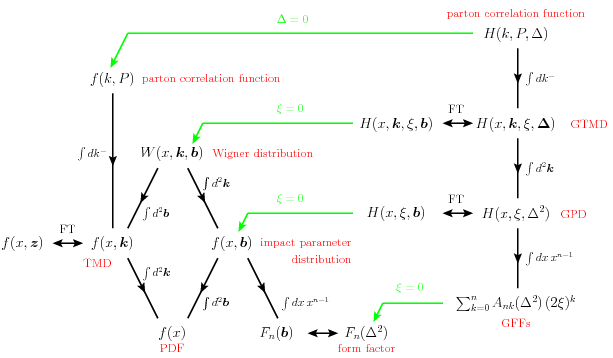
\includegraphics[width=7in]{Chapter1/importfigs/fig6_introGPD_TMD.png}
\par\end{centering}
\caption{Interconnectedness of Parton Distributions \cite{Diehl:2003ny} \label{fig:gpdTMDWeb}}
\end{figure}

TMDs and GPDs manifest non-perturbative QCD effects. The Wigner distribution, at this scale, reflects the relationship between the position and momentum of partons. Integrating the Wigner function over the transverse distance yields the TMD, while integrating over transverse momentum yields a GPD with spatial information. 

Yoshitaka Hatta uses the dipole framework to show that the azimuthal angular correlations of coherent dijets are generated by the underlying Wigner distribution of the small-x gluons. Furthermore, these correlations are consistent with predictions based on standard collinear factorization. Relevant kinematic variables are mapped in the figure \ref{fig:yatta1}. The diagram shows a virtual photon interacting with a nucleon. $k_1$ and $k_2$ are the transverse momenta of the final state jets. These jets originate from a quark-antiquark pair. 

\begin{figure}[h!]
\begin{centering}
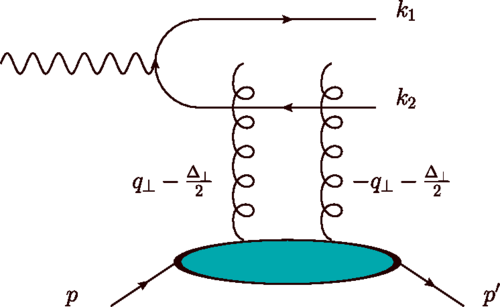
\includegraphics[width=4in]{Chapter1/importfigs/fig4_yatta.png}
\par\end{centering}
\caption{Feynman Diagram of Coherent Dijets in Dipole Framework \cite{Hatta:2016dxp}\label{fig:yatta1}}.
\end{figure}